%% file: template.tex = LaTeX template for article-like report 
%% init: sometime 1993
%% last: Feb  8 2015  Rob Rutten  Deil
%% site: http://www.staff.science.uu.nl/~rutte101/rrweb/rjr-edu/manuals/student-report/

%% First read ``latex-bibtex-simple-manual.txt'' at
%% http://www.staff.science.uu.nl/~rutte101/Report_recipe.html

%% Start your report production by copying this file into your XXXX.tex.
%% Small changes to the header part will make it an A&A or ApJ manuscript.

%%%%%%%%%%%%%%%%%%%%%%%%%%%%%%%%%%%%%%%%%%%%%%%%%%%%%%%%%%%%%%%%%%%%%%%%%%%%
\documentclass{aa}   %% Astronomy & Astrophysics style class

\usepackage{graphicx,natbib,url,twoopt}
\usepackage[varg]{txfonts}           %% A&A font choice
\usepackage{hyperref}                %% for pdflatex
%%\usepackage[breaklinks]{hyperref}  %% for latex+dvips
%%\usepackage{breakurl}              %% for latex+dvips
\usepackage{pdfcomment}              %% for popup acronym meanings
\usepackage{acronym}                 %% for popup acronym meanings

\hypersetup{
  colorlinks=true,   %% links colored instead of frames
  urlcolor=blue,     %% external hyperlinks
  linkcolor=red,     %% internal latex links (eg Fig)
}

\bibpunct{(}{)}{;}{a}{}{,}    %% natbib cite format used by A&A and ApJ

\pagestyle{plain}   %% undo the fancy A&A pagestyle 

%% Add commands to add a note or link to a reference
\makeatletter
\newcommand{\bibnote}[2]{\@namedef{#1note}{#2}}
\newcommand{\biblink}[2]{\@namedef{#1link}{#2}}
\makeatother

%% Commands to make citations ADS clickers and to add such also to refs
%% May 2014: they give error stops ("Illegal parameter number ..."}
%%   for plain latex with TeX Live 2013; the ad-hoc fixes added below let
%%   latex continue instead of stop within these commands.
%%   Please let me know if you know a better fix!
%%   No such problem when using pdflatex.
\makeatletter
 \newcommandtwoopt{\citeads}[3][][]{%
   \nonstopmode%              %% fix to not stop at error message in latex
   \href{http://adsabs.harvard.edu/abs/#3}%
        {\def\hyper@linkstart##1##2{}%
         \let\hyper@linkend\@empty\citealp[#1][#2]{#3}}%   %% Rutten, 2000
   \biblink{#3}{\href{http://adsabs.harvard.edu/abs/#3}{ADS}}%
   \errorstopmode}            %% fix to resume stopping at error messages 
 \newcommandtwoopt{\citepads}[3][][]{%
   \nonstopmode%              %% fix to not stop at error message in latex
   \href{http://adsabs.harvard.edu/abs/#3}%
        {\def\hyper@linkstart##1##2{}%
         \let\hyper@linkend\@empty\citep[#1][#2]{#3}}%     %% (Rutten 2000)
   \biblink{#3}{\href{http://adsabs.harvard.edu/abs/#3}{ADS}}%
   \errorstopmode}            %% fix to resume stopping at error messages
 \newcommandtwoopt{\citetads}[3][][]{%
   \nonstopmode%              %% fix to not stop at error message in latex
   \href{http://adsabs.harvard.edu/abs/#3}%
        {\def\hyper@linkstart##1##2{}%
         \let\hyper@linkend\@empty\citet[#1][#2]{#3}}%     %% Rutten (2000)
   \biblink{#3}{\href{http://adsabs.harvard.edu/abs/#3}{ADS}}%
   \errorstopmode}            %% fix to resume stopping at error messages 
 \newcommandtwoopt{\citeyearads}[3][][]{%
   \nonstopmode%              %% fix to not stop at error message in latex
   \href{http://adsabs.harvard.edu/abs/#3}%
        {\def\hyper@linkstart##1##2{}%
         \let\hyper@linkend\@empty\citeyear[#1][#2]{#3}}%  %% 2000
   \biblink{#3}{\href{http://adsabs.harvard.edu/abs/#3}{ADS}}%
   \errorstopmode}            %% fix to resume stopping at error messages 
\makeatother

%% Acronyms
\newacro{ADS}{Astrophysics Data System}
\newacro{NLTE}{non-local thermodynamic equilibrium}
\newacro{NASA}{National Aeronautics and Space Administration}

%% Add popups with meaning to acronyms 
%% NB: only show up in Adobe Reader and do not work with \input or \include
\gdef\acp#1{%
  \pdfmarkupcomment[markup=Underline,color={1 1 1},author={{#1}},opacity=0]%
  {{#1}}{{\acl{#1}}}}

%% Spectral species
\def\MgI{\ion{Mg}{I}}          %% A&A; for aastex use \def\MgI{\ion{Mg}{1}} 
\def\MgII{\ion{Mg}{II}}        %% A&A; for aastex use \def\MgII{\ion{Mg}{2}} 

%% Hyphenation
\hyphenation{Schrij-ver}       %% Dutch ij is a single character

%%%%%%%%%%%%%%%%%%%%%%%%%%%%%%%%%%%%%%%%%%%%%%%%%%%%%%%%%%%%%%%%%%%%%%%%%%%%
\begin{document}  

%% simple header.  Change into A&A or ApJ commands for those journals

\twocolumn[{%
\vspace*{4ex}
\begin{center}
  {\Large \bf Stellar Spectra B. LTE Line Formation}\\[4ex]       
  {\large \bf Andreas Ellewsen}\\[4ex]
  %{\large \bf Andreas Ellewsen$^{1}$}\\[4ex]
  %\begin{minipage}[t]{15cm}
  %      $^1$ Institute of theoretical astrophysics\\

%  {\bf Abstract.} We learned how to write nice reports \ldots 

  %\vspace*{2ex}
  %\end{minipage}
\end{center}
}] 
%%%%%%%%%%%%%%%%%%%%%%%%%%%%%%%%%%%%%%%%%%%%%%%%%%%%%%%%%%%%%%%%%%%%%%%%%%%%
\section{Stratification of the solar atmosphere}
%%%%%%%%%%%%%%%%%%%%%%%%%%%%%%%%%%%%%%%%%%%%%%%%%%%%%%%%%%%%%%%%%%%%%%%%%%%%
In this exercise we study the radial stratification of the solar atmosphere by using the FALC model by Fontela et al. (1993)

\subsection{FALC density stratification}
The first thing to do is import the data from the modelfiles and make figures of some key quantities.
I start by plotting the total pressure $p_{total}$ against colmn mass $m$. See figures \ref{ptotal} and \ref{ptotal_log}.
We see that they scale linearly. From this we can conclude that we can write 
\begin{equation}
 p_{total} = Cm
\end{equation}
where if one finds $C$ for all pressures and column masses and then find the average $C$, I get $C = g_{surface} = 27398.2$ cm/s$^2$.

% \begin{figure}
%  \includegraphics[width=.49\textwidth]{ptotal.png}
%  \caption{Plot of total pressure against column mass.}
%  \label{ptotal} 
% \end{figure}
% \begin{figure}
%  \includegraphics[width=.49\textwidth]{ptotal_log.png}
%  \caption{Plot of total pressure against column mass using logarithmic scale.}
%  \label{ptotal_log} 
% \end{figure}

Fontena et a. (1993) assumed complete mixing, so we check that this condition holds by plotting the ratio of the hydrogen mass density to the total mass density against height. Next we add the Helium as well and calculate the contribution of helium and hydrogen to the total. From the figure it seems that nearly all of the density is contributed form hydrogen and helium. However if one does the calculation one finds that the average fraction of the remaining elements (the ``metals'') contributes $0.002$ ($0.02 \%$) of the total .This can be seen in figure \ref{Hdensratio_height}
% \begin{figure}
%  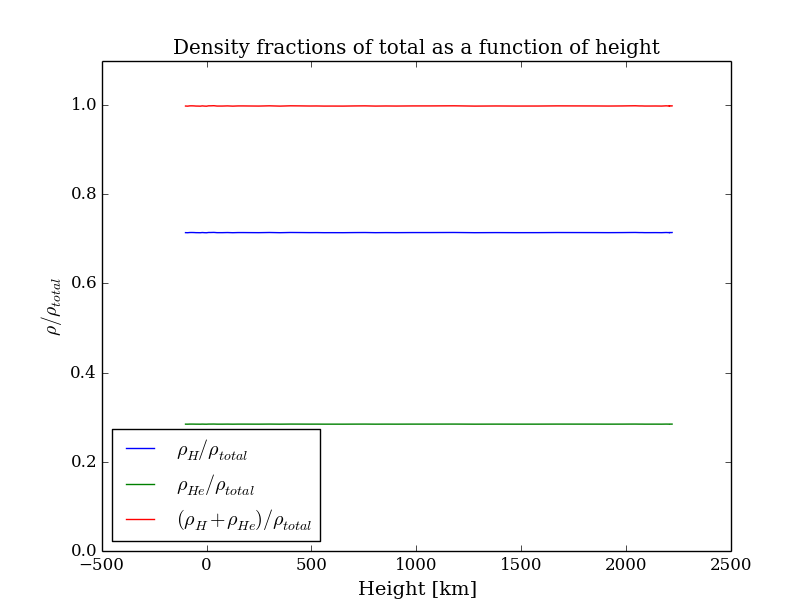
\includegraphics[width=.49\textwidth]{Hdensratio_height.png}
%  \caption{Ratio of hydrogen mass density to total mass density vs height.}
%  \label{Hdensratio_height} 
% \end{figure}

Next we plot the column mass against height. See figure \ref{colm_height}. Note that the curve becomes nearly straight if we make the y-axis logarithmic in figure \ref{colm_height_log}. This is caused by XXXXXXXXXXXXXXXXXXXXXXXXX.
% \begin{figure}
%  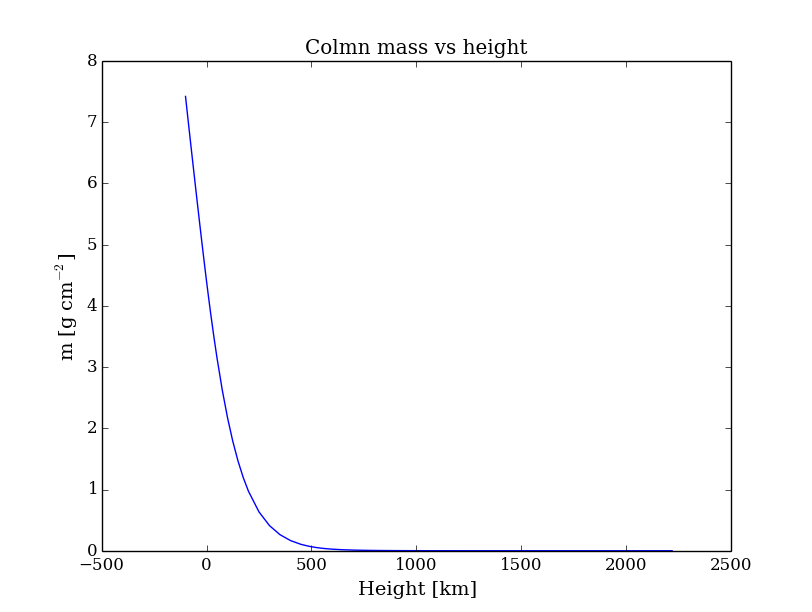
\includegraphics[width=.49\textwidth]{col_height.png}
%  \caption{Column mass vs height.}
%  \label{colm_height} 
% \end{figure}

% \begin{figure}
%  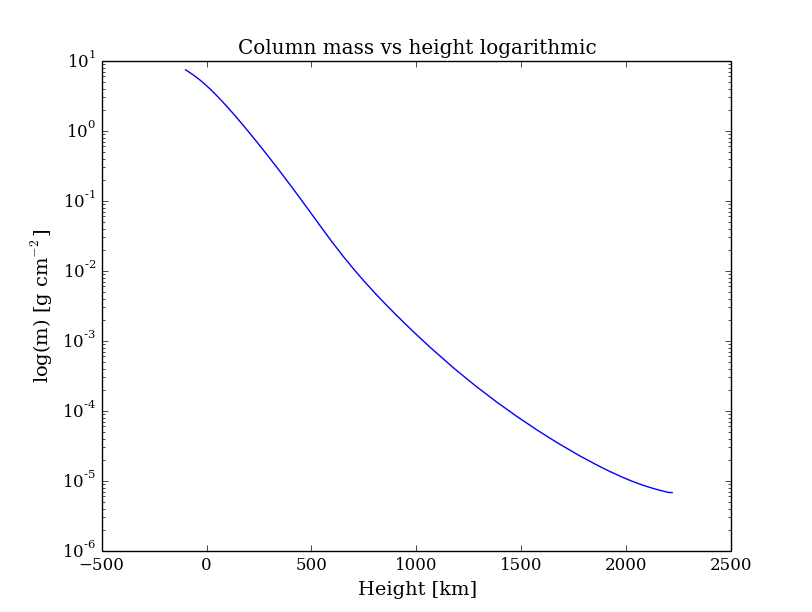
\includegraphics[width=.49\textwidth]{col_height_log.png}
%  \caption{Column mass vs height with logarithimic y-axis.}
%  \label{colm_height_log} 
% \end{figure}

The next quantity to look at is gas density. Gas density is plottes against height in figure \ref{gdens_height}.

% \begin{figure}
%  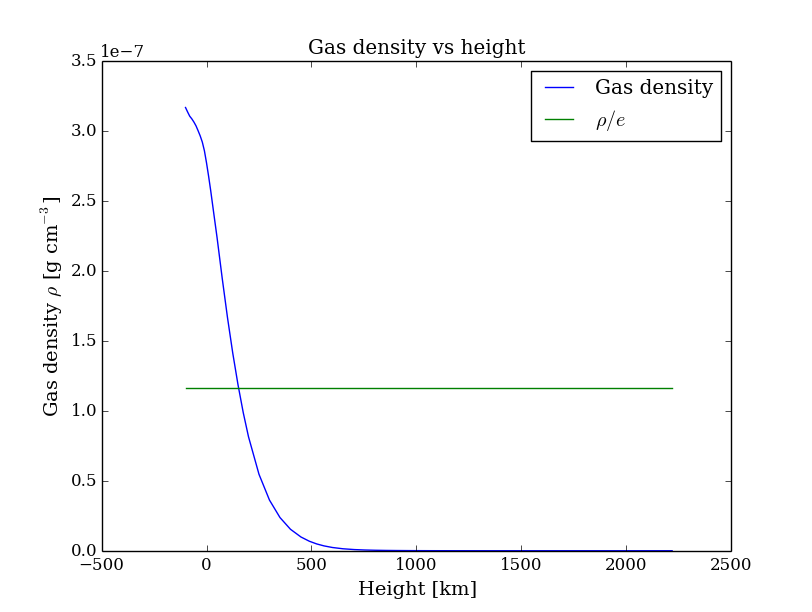
\includegraphics[width=.49\textwidth]{gdens_height.png}
%  \caption{Gas density against height with the point where $\rho = \rho_0/e$ marked with a line.}
%  \label{colm_height_log} 
% \end{figure}

We want to know the pressure scale height $H_\rho$ in  
\begin{equation}
 \rho \approx \rho(0)exp(-h/H_{\rho})
\end{equation}

This can be found from the definition
\begin{equation}
 H_\rho = \frac{kT}{M g}
\end{equation}
where $k$ is boltzmanns constant, T is temperature in K, M is the mean molecular weight, and g is surface gravity.
If one assumes that most of the molecules in the photosphere is hydrogen we can set $M=m_H$. Inserting the values for the deep photosphere ($h = -100$) then gives a scale height of $H_\rho = 196.3$ km. This is not realistic. Assuming that the photosphere only contains helium gives a scale height $H_\rho = 49.3 km$. The real number is somewhere between these two, and thus when ones find the mean molecular weight as a function of height later, one should recalculate this number.

Another way to do this is to just mark the point where the density has fallen to $1/e$ of its original value. In figure \ref{gdens_height} this is marked with a line. The point the two lines cross gives $H_\rho \approx 150 $km.


The next step is to compute the gas pressure and plot it against height. We also overplot the product $(n_H + n_e)kT$. See figure \ref{gas_height}. There is some difference between the curves. Plotting the ratio between the curves shows this clearly (figure \ref{gas_height_ratio}). Note however that the sun does not only contain hydrogen. Because of this we must include the hydrogen number density in the ideal gas law. By doing this we obtain figure \ref{gas_height_hel} which shows a curve that seems to be overlapping perfectly. Plotting the ratio between the two curves shows that it deviates only slightly at the fourth decimal place. See figure \ref{gas_height_hel_ratio}. From this we can conclude that the ideal gas law is a very good approximation.

% \begin{figure}
%  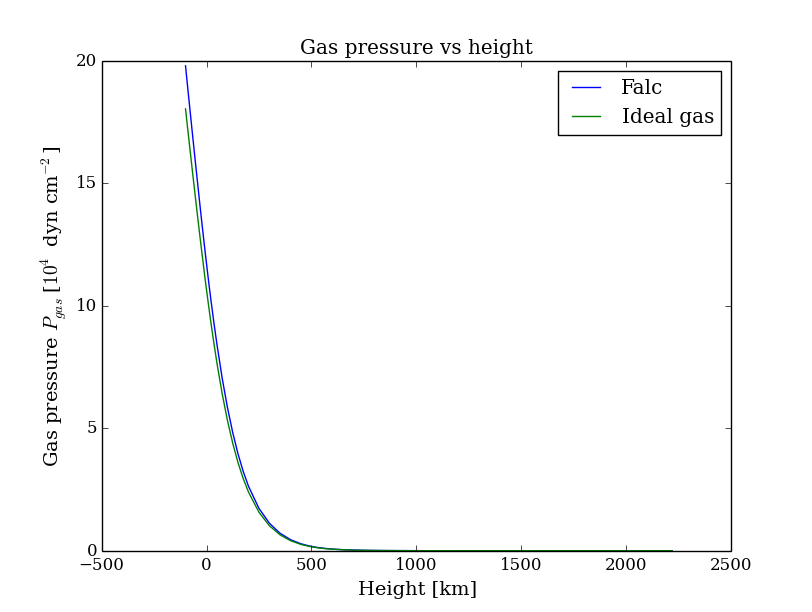
\includegraphics[width=.49\textwidth]{gas_height.png}
%  \caption{Gas pressure against height.}
%  \label{gas_height} 
% \end{figure}

% \begin{figure}
%  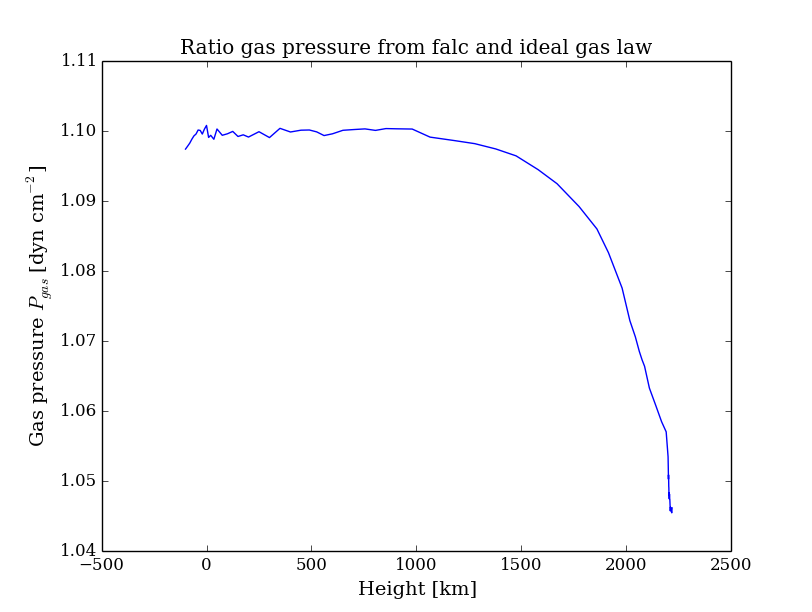
\includegraphics[width=.49\textwidth]{gas_height_ratio.png}
%  \caption{Ratio between gas pressure and ideal gas law.}
%  \label{gas_height_ratio_hel} 
% \end{figure}

% \begin{figure}
%  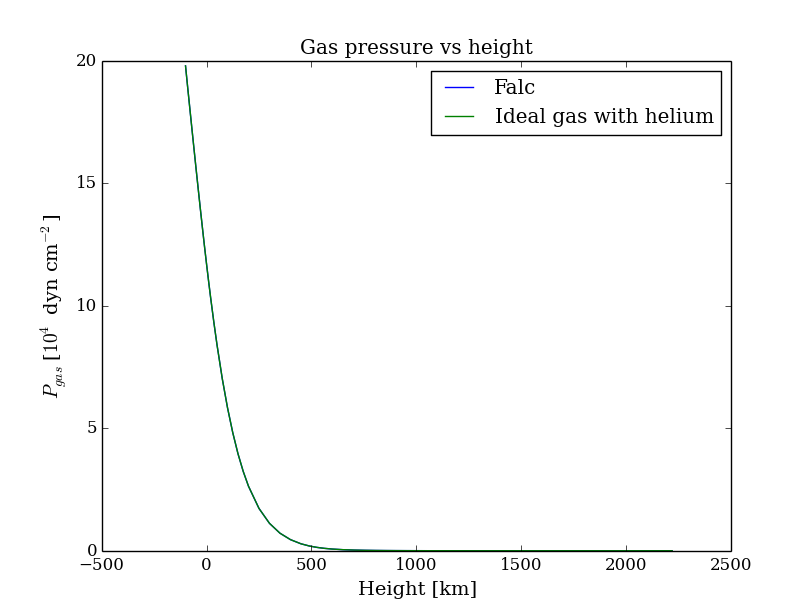
\includegraphics[width=.49\textwidth]{gas_height_hel.png}
%  \caption{Gas pressure against height with helium included in curve forideal gas law.}
%  \label{gas_height} 
% \end{figure}

% \begin{figure}
%  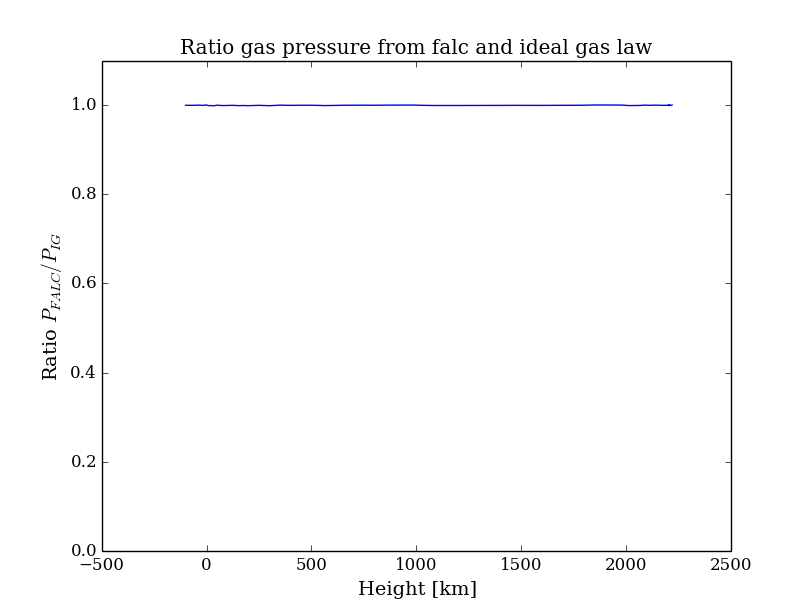
\includegraphics[width=.49\textwidth]{gas_height_ratio_hel.png}
%  \caption{Ratio between gas pressure and ideal gas law when including helium.}
%  \label{gas_height_ratio_hel} 
% \end{figure}

With that done we want to look at the total hydrogen density. We should also include the electron density, proton density, and the density of the electrons that do not result from hydrogen ionization. The electron density, proton density and electron density can be read out of the FALC model. To find the density of the electrons not from ionized hydrogen we need to assume that all of the protons come from ionized hydrogen. This would indicate that $n_H - n_p$ equals the number of neutral hydrogen atoms. And since each neutral hydrogen has one electron this would be the number of electrons still bound to hydrogen, e.g those not from ionized hydrogen. The density of these should then be
\begin{equation}
 n_{be} = (n_H - n_p).
\end{equation}
This is plotted against height in figure \ref{densities_height}. 
% \begin{figure}
%  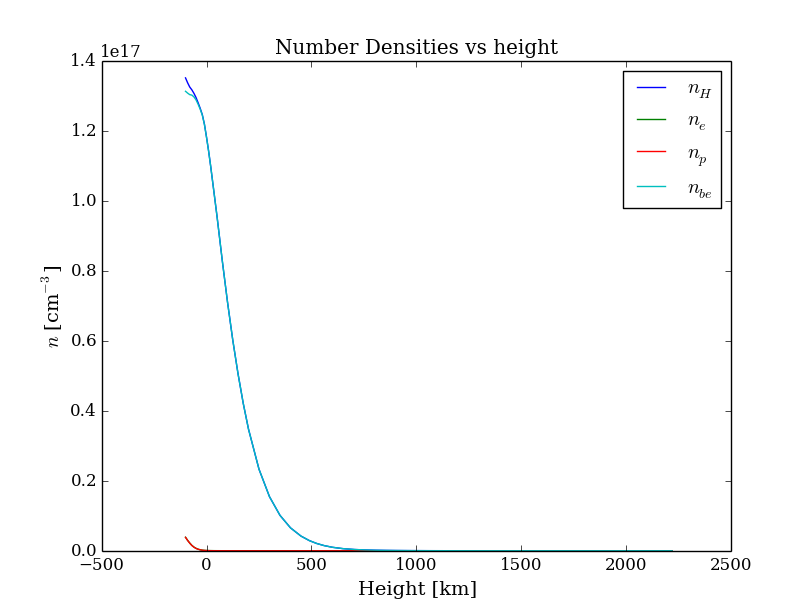
\includegraphics[width=.49\textwidth]{densities_height.png}
%  \caption{Figure shows densities for a number of quantities against height.}
%  \label{densities_height} 
% \end{figure}

From the graph we see that the number density of protons is a little above 0 for very low heights. This indicates that the hydrogen gets ionized at this height. As the height increases this goes to zero indicating that the hydrogen remains neutral when height increases. Because of this it is only logical that the electron density goes to zero as well, and that the density of the elctrons not from ionized hydrogen approaches the density of the hydrogen (since nearly all of the hydrogen is neutral hydrogen). Figure \ref{densities_height_log} shows the same with a logarithmic
% \begin{figure}
%  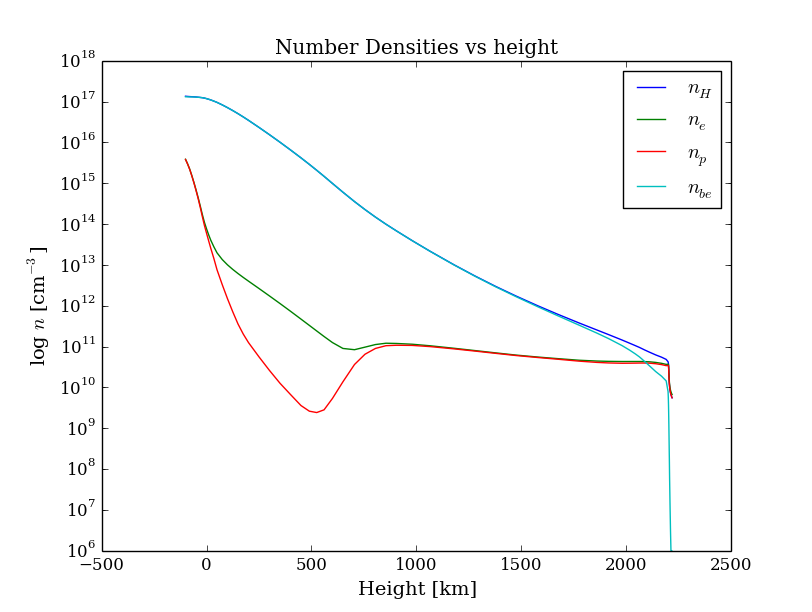
\includegraphics[width=.49\textwidth]{densities_height_log.png}
%  \caption{Figure shows densities for a number of quantities against height with logarithmic y-axis.}
%  \label{densities_height_log} 
% \end{figure}

As the height increases the number density of everything approaches zero, which makes sense since we are looking at the atmosphere of the sun. At some point the should be vacuum.

With that done plot the ionization fraction of hydrogen against height. See figure \ref{hyd_ion}. Note the logarithmic scale.
% \begin{figure}
%  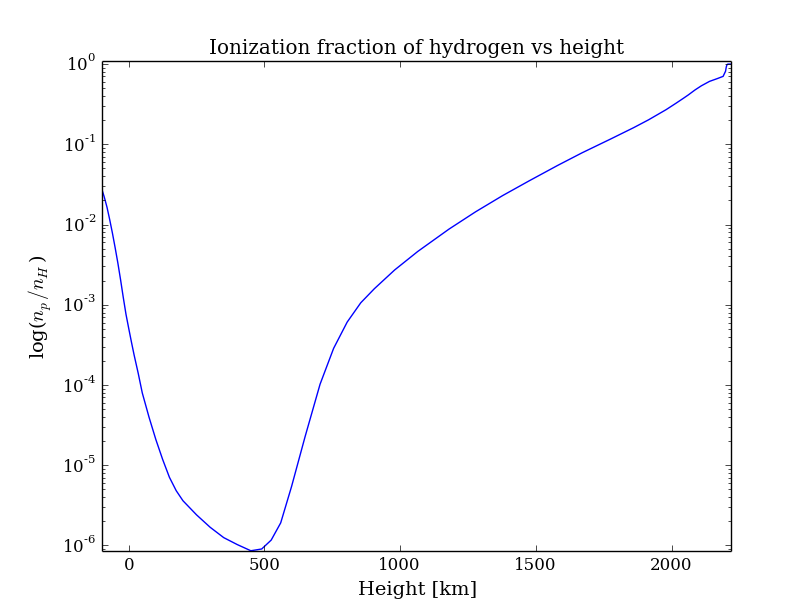
\includegraphics[width=.49\textwidth]{hyd_ion.png}
%  \caption{Figure shows the ionization fraction of hydrogen depending on height in kilometers.}
%  \label{hyd_ion} 
% \end{figure}







%\begin{acknowledgements}
%\end{acknowledgements}

%%%%%%%%%%%%%%%%%%%%%%%%%%%%%%%%%%%%%%%%%%%%%%%%%%%%%%%%%%%%%%%%%%%%%%%%%%%%
%% references
\section{References}
Rutten, R. J.: 1991, The Generation and Transportation of Radiation, Sterrekundig Instuut Utrecht, The Netherlands

%\bibliographystyle{aa-note} %% aa.bst but adding links and notes to references
%\raggedright              %% only for adsaa with dvips, not for pdflatex
%\bibliography{XXX}          %% XXX.bib = your Bibtex entries copied from ADS

\end{document}


